\chapter{Toepassingen van dynamisch programmeren}
\section{Optimale binaire zoekbomen}
\begin{figure}[ht]
    \centering
    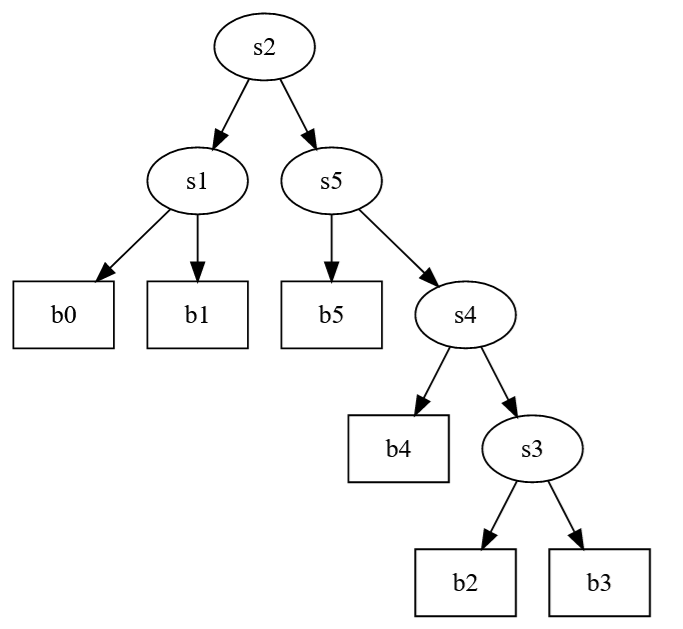
\includegraphics[width=0.5\textwidth]{optimal-binary-tree}
    \caption{Een optimale binaire zoekboom met bijhorende kansentabel.}
    \label{}
\end{figure}

\begin{table}[ht]
    \centering
    \begin{tabular}{l | c c c c c c}
        i & 0 & 1 & 2 & 3 & 4 & 5 \\
        \hline
        $p_i$ & & 0.15 & 0.10 & 0.05 & 0.10 & 0.20 \\
        $q_i$ & 0.05 & 0.10 & 0.05 &0.05 &0.05 & 0.10  
    \end{tabular}
\end{table}
\begin{itemize}
    \item Veronderstel dat de gegevens die in een binaire zoekboom moeten opgeslaan worden op voorhand gekend zijn.
    \item Veronderstel ook dat de waarschijnlijkheid gekend is waarmee de gegevens gezocht zullen worden.
    \item Tracht de boom zo te schikken zodat de verwachtingswaarde van de zoektijd minimaal wordt.
    \item De zoektijd wordt bepaald door de lengte van de zoekweg.
    \item De gerangschikte sleutels van de $n$ gegevens zijn $s_1, \dots, s_n$.
    \item De $n + 1$ bladeren zijn $b_0, \dots, b_n$.
    \begin{itemize}
        \item Elk blad staat voor een afwezig gegeven die in een deelboom op die plaats had moeten zitten.
        \item Het blad $b_0$ staat voor alle sleutels kleiner dan $s_1$.
        \item Het blad $b_n$ staat voor alle sleutels groter dan $s_n$.
        \item Het blad $b_i$ staat voor alle sleutels gorter dan $s_i$ en kleiner dan $s_{i +1}$, met $1 \leq i < n$
    \end{itemize}
    \item De waarschijnlijkheid om de $i$-de sleutel $s_i$ te zoeken is $p_i$. 
    \item De waarschijnlijkheid om alle afwezige sleutels, voorgesteld door een blad $b_i$, te zoeken is $q_i$.
    \item De som van alle waarschijnlijkheden moet 1 zijn:
    $$\sum_{i = 1}^n p_i + \sum_{i = 0}^n q_i = 1$$
    \item Als de zoektijd gelijk is aan het aantal knopen op de zoekweg (de diepte plus één), dan is de verwachtingswaarde van de zoektijd van een binaire boom
    $$\sum_{i = 1}^n p_i (\hbox{diepte}(s_i) + 1) + \sum_{i = 0}^n q_i (\hbox{diepte}(b_i) + 1)$$
    \item Deze verwachtingswaarde moet geminimaliseerd worden.
    \begin{itemize}
        \item Boom met minimale hoogte is niet voldoende.
        \item Alle mogelijke zoekbomen onderzoeken is ook geen optie, hun aantal is 
        \begin{align*}
            \frac{1}{n + 1}\binom{2n}{n} & \sim \frac{1}{n + 1} \cdot \frac{2^{2n}}{\sqrt{\pi n}} \\
                                         & \sim \frac{1}{n + 1} \cdot \frac{4^{n}}{\sqrt{\pi n}} \\
                                         & \sim \Omega\bigg(\frac{4^n}{n\sqrt{n}}\bigg)
        \end{align*}
        \good Dynamisch programmeren biedt een uitkomst.
    \end{itemize}
    \item Een optimalisatieprobleem komt in aanmerkingen voor een efficiënte oplossing via dynamisch programmeren als het:
    \begin{enumerate}
        \item het een \textbf{optimale deelstructuur} heeft;
        \item de \textbf{deelproblemen onafhankelijk maar overlappend} zijn.
    \end{enumerate}
    \item Is dit hier van toepassing?
    \begin{itemize}
        \item Is er een optimale deelstructuur?
        \begin{itemize}
            \item Als een zoekboom optimaal is, moeten zijn deelbomen ook optimaal zijn.
            \item Een optimale oplossing bestaat uit optimale oplossingen voor deelproblemen.
        \end{itemize}
        \item Zijn de deelproblemen onafhankelijk?
        \begin{itemize}
            \item Ja want deelbomen hebben geen gemeenschappelijke knopen.
        \end{itemize}
        \item Zijn de deelproblemen overlappend?
        \begin{itemize}
            \item Elke deelboom bevat een reeks opeenvolgende sleutels $s_i, \dots s_j$ met bijhorende bladeren $b_{i - 1}, \dots, b_j$.
            \item Deze deelboom heeft een wortel $s_w$ waarbij $(i \leq w \leq j)$.
            \item De linkse deelboom bevat de sleutels $s_i, \dots, s_{w - 1}$ en bladeren $b_{i - 1}, \dots, b_{w - 1}$.
            \item De rechtse deelboom bevat de sleutels $_{w + 1}, \dots, s_j$ en bladeren $b_{w}, \dots, b_j$.
            \item Voor een optimale deelboom met wortel $s_w$ moeten deze beide deelbomen ook optimaal zijn.
            \item Deze wordt gevonden door:
            \begin{enumerate}
                \item achtereenvolgens elk van zijn sleutels $s_i, \dots, s_j$ als wortel te kiezen;
                \item de zoektijd voor de boom te berekenen door gebruikte maken van de zoektijden van de optimale deelbomen;
                \item de wortel te kiezen die de kleinste zoektijd oplevert.
            \end{enumerate} 
        \end{itemize}
    \end{itemize}
    \item De kleinst verwachte zoektijd van een boom met sleutels $s_i, ..., s_j$ is $z(i, j)$ en moet voor elke deelboom bepaald worden, dus voor alle $i$ en $j$ waarbij:
    \begin{itemize}
        \item $1 \leq i \leq n + 1$
        \item $i - 1 \leq j \leq n$
    \end{itemize}
    \item De optimale boom heeft dus de kleinste verwachte zoektijd $z(1, n)$.
    \item Hoe $z_w(i, j)$ bepalen voor een deelboom met wortel $s_w$?
    \begin{itemize}
        \item Gebruik de kans om in de wortel te komen.
        \item Gebruik de optimale zoektijden van zijn deelbomen, $z(i, w - 1)$ en $z(w + 1, j)$.
        \item Gebruik ook de diepte van elke knoop, maar elke knoop staat nu op een niveau lager. 
        \begin{itemize}
            \item De bijdrage tot de zoektijd neemt toe met de som van de zoekwaarschijnlijkheden.
            $$g(i, j) = \sum_{k = i}^{j} p_k + \sum_{k = i - 1}^{j} q_k$$
        \end{itemize}
        \item Hieruit volgt:
        \begin{align*}
            z_w(i, j) & = p_w + (z(i, w - 1) + g(i, w - 1)) + (z(w + 1, j) + g(w + 1, j)) \\
                      & = z(i , w - 1) + z(w + 1, j) + g(i, j)
        \end{align*}
    \end{itemize}
    \item Dit moet minimaal zijn $\rightarrow$ achtereenvolgens elke sleutel van de deelboom tot wortel maken.
    \begin{itemize}
        \item De index $w$ doorloopt alle waarden tussen $i$ en $j$.
        \begin{align*}
            z(i, j) & = \min_{i \leq w \leq j} \{ z_w(i, j)\} \\
                    & = \min_{i \leq w \leq j} \{ z(i , w - 1) + z(w + 1, j)\}  + g(i, j)
        \end{align*}
    \end{itemize}
    \item Hoe wordt de optimale boom bijgehouden?
    \begin{itemize}
        \item Hou enkel de index $w$ bij van de wortel van elke optimale deelboom.
        \item Voor de deelboom met sleutels $s_i, \dots, s_j$ is  de index $w = r(i, j)$.
    \end{itemize}
    \item Implementatie:
    \begin{itemize}
        \item Een recursieve implementatie zou veel deeloplossingen opnieuw berekenen.
        \item Daarom \textbf{bottom-up} implementeren. Maakt gebruik van drie tabellen:
        \begin{enumerate}
            \item Tweedimensionale tabel $z[1..n + 1, 0..n]$ voor de waarden $z(i, j)$.
            \item Tweedimensionale tabel $g[1..n + 1, 0..n]$ voor de waarden $g(i, j)$.
            \item Tweedimensionale tabel $r[1..n, 1..n]$ voor de indices $r(i, j)$.
            
        \end{enumerate}
        \item Algoritme:
        \begin{enumerate}
            \item Initialiseer de waarden $z(i, i-1)$ en $g(i, i-1)$ op $q[i - 1]$.
            \item Bepaal achtereenvolgens elementen op elke evenwijdige diagonaal, in de richting van de tabelhoek linksboven.
            \begin{itemize}
                \item Voor $z(i, j)$ zijn de waarden $z(i, i-1), z(i, i), \dots, z(i, j-1)$ van de linkse deelboom nodig en de waarden $z(i + 1, j), \dots, z(j, j), z(j + 1, j)$ van de rechtse deelbom nodig.
                \item Deze waarden staan op diagonalen onder deze van $z(i, j)$.
            \end{itemize}
        \end{enumerate}
    \end{itemize}

    \item Efficiëntie:
    \begin{itemize}
        \item \textbf{Bovengrens:} drie verneste lussen $\rightarrow O(n^3)$.
        \item \textbf{Ondergrens:} \begin{itemize}
            \item Meeste werk bevindt zich in de binneste lus.
            \item Een deelboom met sleutels $s_i, \dots s_j$ heeft $j - i + 1$ mogelijke wortels.
            \item Elke test is $O(1)$.
            \item Dit werk is evenredig met
            \begin{align*}
                            & \sum_{i = 1}^n\sum_{j = i}^n (j - i + 1) \\
                \Rightarrow \qquad& \sum_{i = 1}^n i^2 \\
                \Rightarrow \qquad& \frac{n(n+1)(2n + 1)}{6} \\
                \Rightarrow \qquad& \Omega(n^3)
            \end{align*}
          
        \end{itemize}
        \item \textbf{Algemeen:} $\Theta(n^3)$.
        \item Kan met een bijkomende eigenschap (zien we niet in de cursus) gereduceerd worden tot $\Theta(n^2)$.
    \end{itemize}
\end{itemize}

\section{Langste gemeenschappelijke deelsequentie}
\begin{itemize}
    \item Een deelsequentie van een string wordt bekomen door nul of meer stringelementen weg te laten.
    \item Elke deelstring is een deelsequentie, maar niet omgekeerd.
    \item Een langste gemeenschappelijke deelsequentie (LGD) van twee strings kan nagaan hoe goed deze twee strings op elkaar lijken.
    \item Geven twee strings:
    \begin{itemize}
        \item $X = \langle x_0, x_1, \dots, x_{n - 1}\rangle$
        \item $Y = \langle y_0, y_1, \dots, y_{m - 1}\rangle$
    \end{itemize}
    \item Hoe LGD bepalen?
    \begin{itemize}
        \item Is er een optimale deelstructuur?
        \begin{itemize}
            \item De deelproblemen zijn paren prefixen van de twee strings. De oplossing bij elk deelprobleem is de lengte van de langst gemeenschappelijke deelsequentie van deze twee prefixen.
            \item Het prefix van $X$ met lengte $i$ is $X_i$.
            \item Het prefix van $Y$ met lengte $j$ is $Y_j$.
            \item De ledige prefix is $X_0$ en $Y_0$.
        \end{itemize}
        \item Zijn de deelproblemen onafhankelijk?
        \begin{itemize}
            \item Stel $Z = \langle z_0, z_1, \dots, z_{k - 1} \rangle$ de LGD van $X$ en $Y$. Er zijn drie mogelijkheden:
            \begin{enumerate}
                \item Als $n = 0$ of $m = 0$ dan is $k = 0$.
                \item Als $x_{n - 1} = y_{m - 1}$ dan is $z_{k - 1} = x_{n - 1} = y_{m - 1}$ en is $Z$ een LGD van $X_{n - 1}$ en $Y_{m - 1}$.
                \item Als $x_{n - 1} \neq y_{m - 1}$ dan is $Z$ een LGD van $X_{n - 1}$ en $Y$ of een LGD van $X$ en $Y_{m - 1}$.
            \end{enumerate}
        \end{itemize}
        \item Zijn de deelproblemen overlappend?
        \begin{itemize}
            \item Om de LGD van $X$ en $Y$ te vinden is het nodig om zowel de LGD van $X$ en $Y_{m - 1}$ als van $X_{n - 1}$ en $Y$ te vinden.
        \end{itemize}
    \end{itemize}
    \item De lengte $c[i, j]$ van de LGD van $X_i$ en $Y_j$ wordt door een recursieve vergelijking bepaald:
    $$c[i, j] = \begin{cases}
        0 & \hbox{als}\; i = 0\;\hbox{of}\; j = 0 \\
        c[i - 1, j - 1] + 1 & \hbox{als}\; i >0\;\hbox{en}\; j > 0\;\hbox{en}\; x_i = y_j\\
        \max(c[i, j- 1], c[i - 1, j]) & \hbox{als}\; i >0\;\hbox{en}\; j > 0\;\hbox{en}\; x_i \neq y_j\\
    \end{cases}$$
    \item De lengte van de LGD komt overeen met $c[n, m]$.
    \item De waarden $c[i, j]$ kunnen eenvoudig per rij van links naar rechts bepaald worden door de recursierelatie.
    \item Efficiëntie:
    \begin{itemize}
        \item We beginnen de tabel in te vullen vanaf $c[1, 1]$ (als $i = 0$ of $j = 0$ zijn de waarden 0).
        \item De tabel $c$ wordt rij per rij, kolom per kolom ingevuld.
        \item De vereiste plaats en totale performantie is beiden $\Theta(nm)$.
    \end{itemize}

\end{itemize}
